\chapter{Generating an EnergyPlus Line Diagram}\label{generating-an-energyplus-line-diagram}

The following list of steps will outline the process for converting an engineering line diagram into an EnergyPlus line diagram. Throughout the process, the components in the systems should be identified and named properly. It is easier to input the system if a list of components and their names is available.

1.~~~~\textbf{Obtain an engineering line diagram for the system.}

2.~~~~\textbf{Identify all the loops in the system.} Some systems may be very complex, but an effort should be made to separate the system into its constituent plant loops. A system may have multiple plant loops. Therefore, proper documentation of the loops and their components should be a priority.

3.~~~~\textbf{Identify the demand side and supply side of the individual loops.} EnergyPlus expects the demand side loop and supply side loop to be entered separately. Some examples of simple plant loops are: a hot water heater (supply component) connected to a heating coil (demand component), a chiller (supply component) connected to a cooling coil (demand component) or a cooling tower (supply component) connected to a water cooled chiller (demand component). These loops may have multiple supply components and multiple demand components. A chiller may also be a supply or demand component depending on the loop.

4.~~~~\textbf{Identify the components in the system.} All the operating/active components, such as chillers, pumps, cooling towers, thermal energy storage tanks, heating and cooling coils, and other components should be identified and named properly. It should be noted that even though EnergyPlus has objects for modeling valves, they are not often used. Instead the flow through a component is regulated by using schedules, plant equipment operation schemes and set points. Passive components such as inlet and outlet pipes for each side of the loop should also be identified, as they will help in modeling the loop connectors.

5.~~~~\textbf{Identify all the nodes in the system.} Nodes are necessary to connect the different components in the system. Nodes define the starting and ending points of branches as well as intermediate nodes on multi-component branches. A good method to pin-point nodes on the line diagram would be to put a node on either side of an active or passive component. Note: If the outlet of one component does not feed into a splitter or a mixer, then the outlet node will be the same as the inlet node of the downstream component.

6.~~~~\textbf{Identify all the branches in the loops.} A good way to define a branch would be to include at least one of the components in the branch. Branches can accommodate multiple components in series, but parallel components should be modeled on separate branches. Operating/active components (except pumps) should be bypassed by adding a bypass branch parallel to the branch containing the active component. Multiple bypass branches in parallel can be replaced by a single bypass branch.

7.~~~~\textbf{Identify the position of the connectors in the system.} Connectors are an integral part of the system and are important in constructing the loop. There are two types of connectors, splitters and mixers. Splitters can distribute the flow from a single branch into multiple parallel branches. Mixers can combine the flow from multiple branches into a single branch. As mentioned above, most systems have multiple supply and demand side components, so splitters and mixers play a crucial role in distributing and recombining the flow of the working fluid through all the components.

8.~~~~\textbf{Generate an EnergyPlus diagram} of the whole system as well as the individual loops by using the information gathered from the preceding steps.

A flowchart for this process is provided in Figure~\ref{fig:flowchart-for-energyplus-line-diagram} .

\begin{figure}[hbtp] % fig 2
\centering
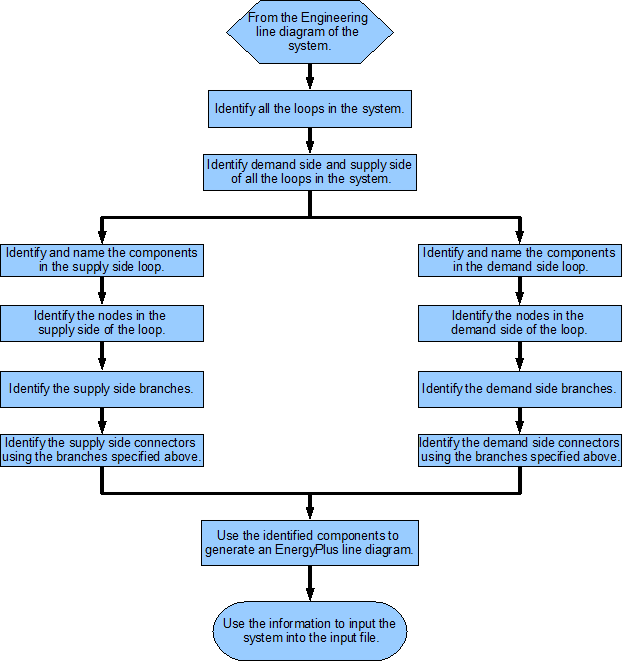
\includegraphics[width=0.9\textwidth, height=0.9\textheight, keepaspectratio=true]{media/image002.png}
\caption{Flowchart for EnergyPlus line diagram generation \protect \label{fig:flowchart-for-energyplus-line-diagram}}
\end{figure}
